\section{Problem No.2} \label{sec:prob2}
\subsection{Problem Description:} 
Write a program to solve the linear advection equation,
$$
u_{t}+au_{x}=0
$$
on the unit interval using a finite volume method of the form
$$
u_{j}^{n+1} = u_{j}^{n} - \frac{\Delta t}{\Delta x}(F_{j+\frac{1}{2}} -F_{j-\frac{1}{2}})
$$
Use the numerical flux function 
$$
F_{j-\frac{1}{2}} = F_{j-\frac{1}{2}}^{up} + \frac{|a|}{2}(1-|\frac{a\Delta t}{\Delta x}|)\delta_{j-\frac{1}{2}}
$$
where $F_{j-\frac{1}{2}}^{up}$ is the upwinding flux,
$$
F_{j-\frac{1}{2}}^{up}=\begin{cases}
         			au_{j-1}\;\;\; if \;\; a> 0\\
         			au_{j}\;\;\; if \;\; a< 0
         			\end{cases}
$$

and $\delta_{j-\frac{1}{2}}$ i the limited difference. Let $\Delta u_{j-\frac{1}{2}} = u_{j}-u_{j-1}$ denote the jump in $u$ across the edge at $x_{j-\frac{1}{2}}$. The limited difference is 
$$
\delta_{j-\frac{1}{2}} = \phi(\theta_{j-\frac{1}{2}})\Delta u_{j-\frac{1}{2}}
$$
where 
$$
\theta_{j-\frac{1}{2}} = \frac{\Delta u_{J_{up}-\frac{1}{2}}}{\Delta u_{j-\frac{1}{2}}}
$$

$$
J_{up} = \begin{cases}
         j-1\;\;\; if \;\; a> 0\\
         j+1\;\;\; if \;\; a< 0
         \end{cases}
$$
Note that you will need two ghost cells on each end of the domain. Write your program so that you may choose from the different limiter functions listed below. 
\\
Upwinding  $\;\; \phi(\theta)=0$\\
\protect{\lw} $\;\; \phi(\theta)=1$\\
\protect{\bw} $\;\; \phi(\theta)=\theta$\\
minmod $\;\; \phi(\theta)=minmod(1,\theta$)\\
superbee $\;\; \phi(\theta)=max(0,min(1,2\theta),min(2,\theta))$\\
MC $\;\; \phi(\theta)=max(0,min((1+\theta)/2,2,2\theta))$\\
van Leer $\;\; \phi(\theta)=\frac{\theta+|\theta|}{1+|\theta|}$\\
The first three are linear methods that we have already studied, and the last four are high resolution methods. 

Solve the advection equation with $a=1$ with periodic boundary conditions for the different initial conditions listed below until time $t=5$ at Courant number 0.9.
\begin{enumerate}
\item Wave packet: $u(x,0)=cos(16\pi x)exp(-50(x-0.5)^2)$
\item Smooth, low frequency: $u(x,0)=sin(2\pi x)sin(4\pi x)$
\item Step function: $$u(x,0)\begin{cases}
							1 \;\;\; if |x-\frac{1}{2}|<\frac{1}{4}\\
							0 \;\;\; otherwise
							\end{cases}$$						
\end{enumerate}
Compare the results with the exact solution, and comment on the solutions generated by the different methods. How do the different high-resolution methods perform in the different test? What high-resolution method would you choose to use in practice?
\subsection{Solution:}
Figure \ref{fig:sol_wave}, \ref{fig:sol_low} and \ref{fig:sol_step} show the solution obtained from solving the above defined finite volume method and flux functions. The comparison between the computed solution and exact one is also shown. 

\begin{figure}[!tbh]
 \centering     
   \subfloat [Upwinding]{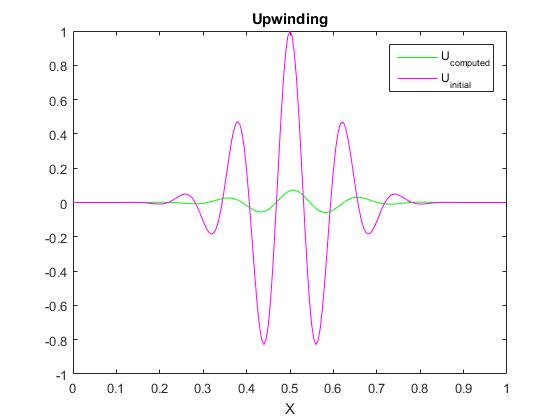
\includegraphics[width=0.3\textwidth]{fig/p2/wave_up.jpg}}
   \subfloat [Lax-Wendroff]{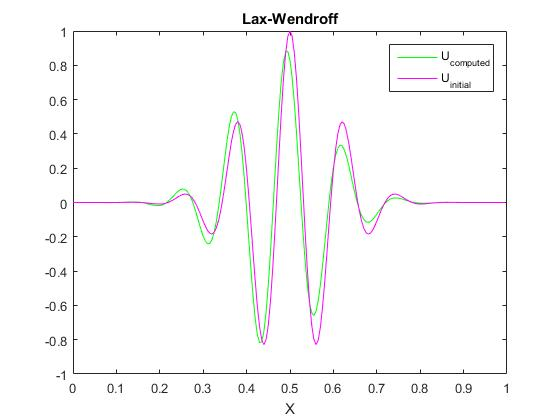
\includegraphics[width=0.3\textwidth]{fig/p2/wave_lw.jpg}}
   \subfloat [Beam-Warming]{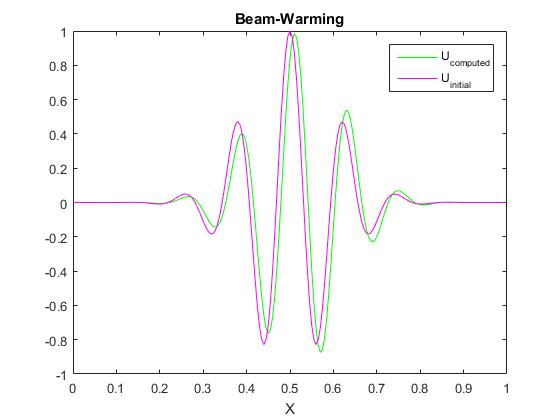
\includegraphics[width=0.3\textwidth]{fig/p2/wave_bw.jpg}}
   
   \subfloat [MC]{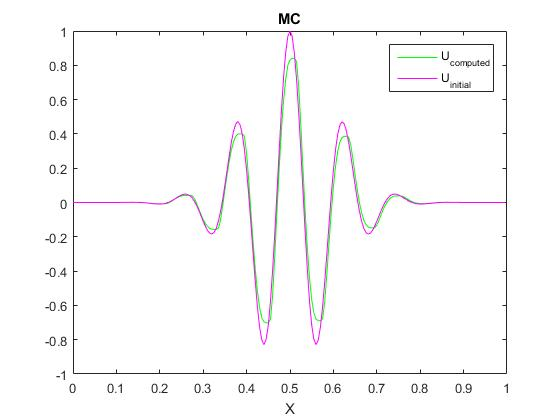
\includegraphics[width=0.25\textwidth]{fig/p2/wave_mc.jpg}}
   \subfloat [Minmod]{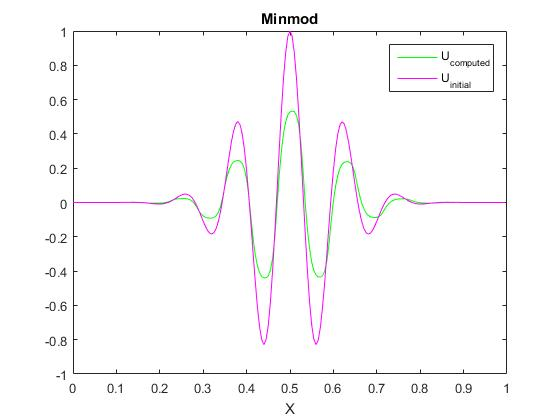
\includegraphics[width=0.25\textwidth]{fig/p2/wave_minmod.jpg}}
   \subfloat [Superbee]{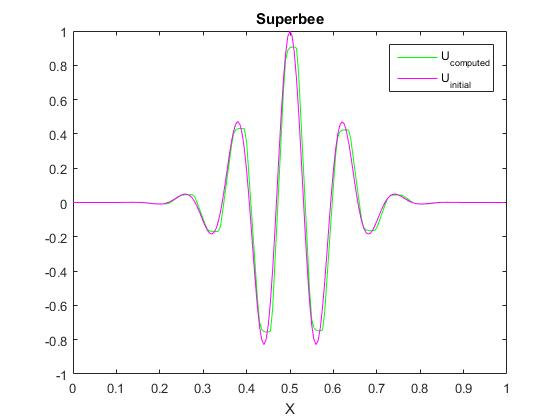
\includegraphics[width=0.25\textwidth]{fig/p2/wave_superbee.jpg}}
   \subfloat [van Leer]{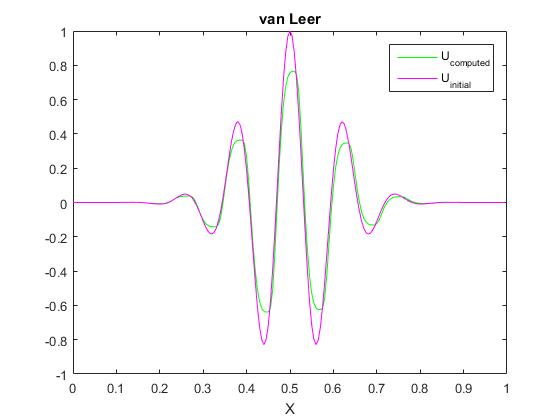
\includegraphics[width=0.25\textwidth]{fig/p2/wave_vanleer.jpg}}
     \caption{Solution using wave packet initial conditions with different limiter functions; green is the computed solution, magenta is   the exact solution.}
   \label{fig:sol_wave}
\end{figure} 
   
   
\begin{figure}[!tbh]
 \centering     
   \subfloat [Upwinding]{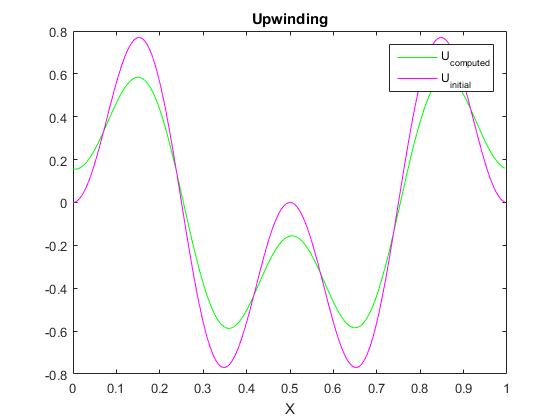
\includegraphics[width=0.3\textwidth]{fig/p2/low_up.jpg}}
   \subfloat [Lax-Wendroff]{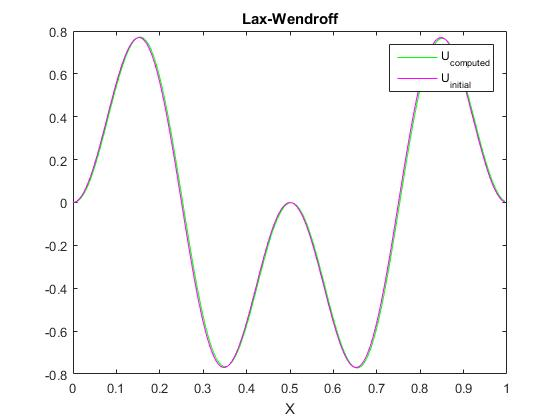
\includegraphics[width=0.3\textwidth]{fig/p2/low_lw.jpg}}
   \subfloat [Beam-Warming]{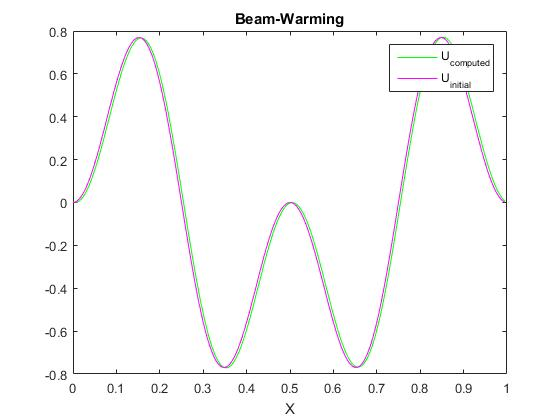
\includegraphics[width=0.3\textwidth]{fig/p2/low_bw.jpg}}
   
   \subfloat [MC]{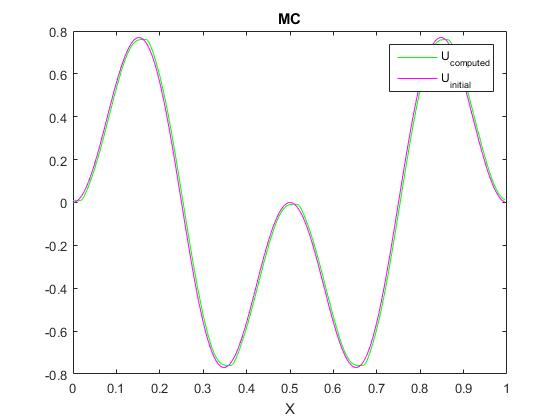
\includegraphics[width=0.25\textwidth]{fig/p2/low_mc.jpg}}
   \subfloat [Minmod]{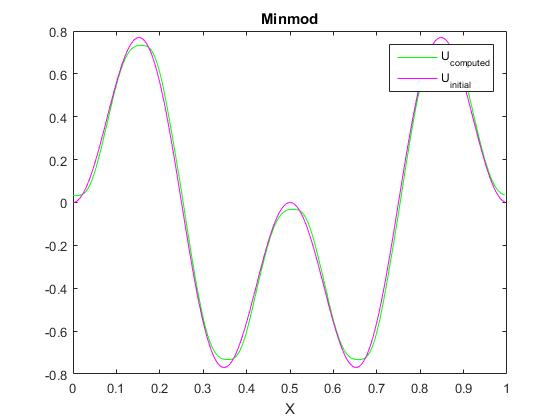
\includegraphics[width=0.25\textwidth]{fig/p2/low_minmod.jpg}}
   \subfloat [Superbee]{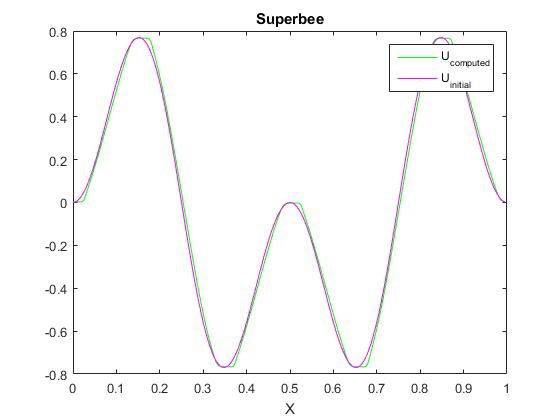
\includegraphics[width=0.25\textwidth]{fig/p2/low_superbee.jpg}}
   \subfloat [van Leer]{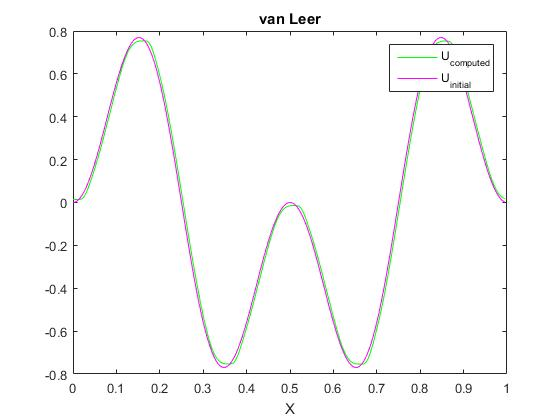
\includegraphics[width=0.25\textwidth]{fig/p2/low_vanleer.jpg}}
     \caption{Solution using smooth, low frequency initial conditions with different limiter functions; green is the computed solution, magenta is   the exact solution.}
   \label{fig:sol_low}
\end{figure}    
   
   
      
\begin{figure}[!tbh]
 \centering     
   \subfloat [Upwinding]{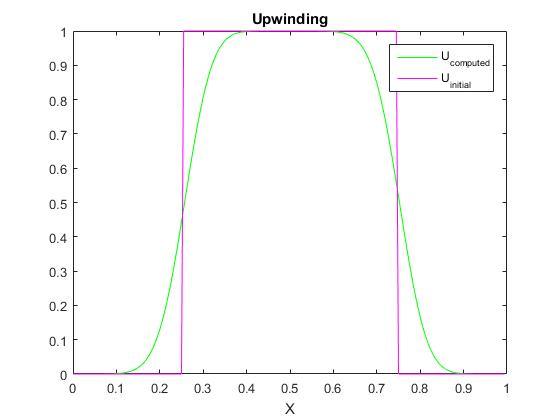
\includegraphics[width=0.3\textwidth]{fig/p2/step_up.jpg}}
   \subfloat [Lax-Wendroff]{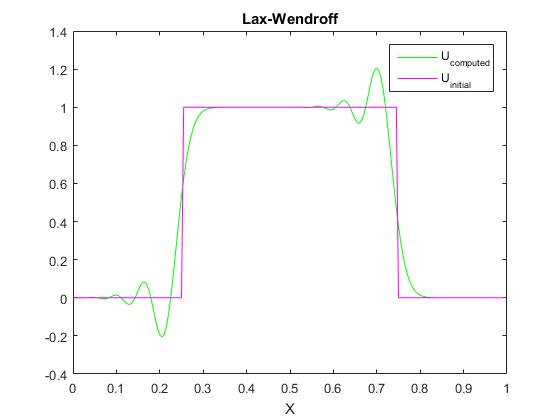
\includegraphics[width=0.3\textwidth]{fig/p2/step_lw.jpg}}
   \subfloat [Beam-Warming]{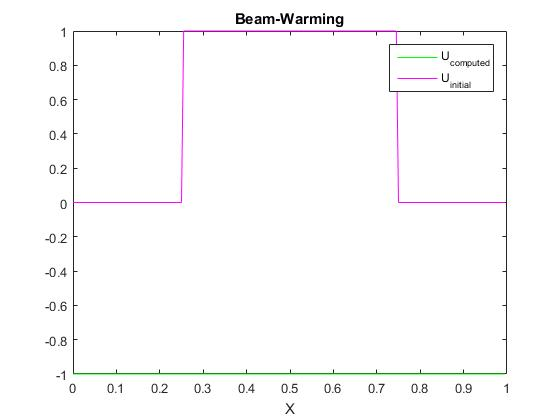
\includegraphics[width=0.3\textwidth]{fig/p2/step_bw.jpg}}
   
   \subfloat [MC]{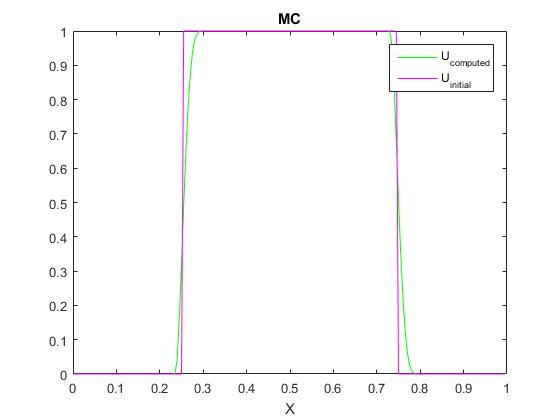
\includegraphics[width=0.25\textwidth]{fig/p2/step_mc.jpg}}
   \subfloat [Minmod]{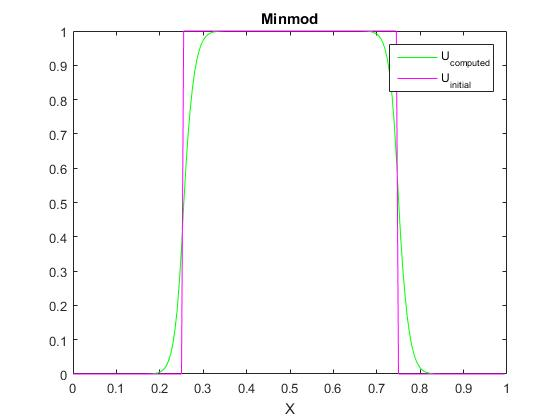
\includegraphics[width=0.25\textwidth]{fig/p2/step_minmod.jpg}}
   \subfloat [Superbee]{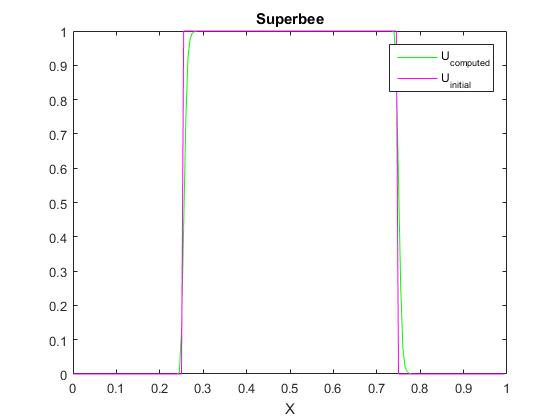
\includegraphics[width=0.25\textwidth]{fig/p2/step_superbee.jpg}}
   \subfloat [van Leer]{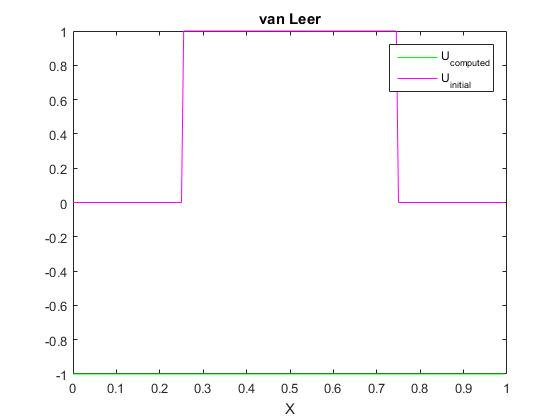
\includegraphics[width=0.25\textwidth]{fig/p2/step_vanleer.jpg}}
     \caption{Solution using step function initial conditions with different limiter functions; green is the computed solution, magenta is   the exact solution.}
   \label{fig:sol_step}
\end{figure} 


For the wave packet initial conditions, Upwinding method shows large diffusion but there is no shift in the solution. \protect{\lw} shows a little diffusion plus a shift to the left while \protect{\bw} has its shift to the right. MC, Superbee, Minmod and van Leer all have diffusion with no shift. Minmod has the largest diffuse while Superbee has the least diffuse. Thus, for smooth initial data, I would choose Superbee. 

For the smooth, low frequency initial conditions, Upwinding shows the same diffuse while \protect{\lw} and \protect{\bw} have a barely noticeable shift (to left and to right respectively). No shift exist for the high-resolution methods. For Minmod, small amount of diffusion was observed near the crests. For Superbee, the solution is less smooth at the crests. Thus, I would choose MC or van Leer for this initial conditions as a high-resolution methods. If non-high resolution method was to be picked, I would pick \protect{\lw} or \protect{\bw}.

For the step function, there sounds to be an error in the solution of both \protect{\bw} and van Leer. It was expected that \protect{\lw} to have ripples that are larger than that for \protect{\lw}. For van Leer, it was expected to be similar to MC for such step function. Upwinding has no ripples but the function got diffused. \protect{\lw} has ripples around the corners but less diffusive than Upwinding. MC has no ripples and it matches closely the exact solution. Same thing goes for Superbee where the solution is even closer to the exact one. Minmode has also no ripples but it is no better than Superbee. Thus, for step/discontinuous initial conditions, I would pick Superbee.  